%%% template.tex
%%%
%%% This LaTeX source document can be used as the basis for your technical
%%% paper or abstract.

%%% The parameter to the ``documentclass'' command is very important.
%%% - use ``review'' for content submitted for review.
%%% - use ``preprint'' for accepted content you are making available.
%%% - use ``tog'' for technical papers accepted to the TOG journal and
%%%   for presentation at the SIGGRAPH or SIGGRAPH Asia conference.
%%% - use ``conference'' for final content accepted to a sponsored event
%%%   (hint: If you don't know, you should use ``conference.'')

\documentclass[review]{acmsiggraph}
\usepackage{amsmath}
\usepackage{amssymb}
\usepackage{wasysym}
\usepackage[scaled=.92]{helvet}
\usepackage{times}
\usepackage{graphicx}
\usepackage{parskip}
\usepackage{url}
\usepackage[labelfont=bf,textfont=it]{caption}
\usepackage{color}
\usepackage{algorithm}
\usepackage{algorithmic}
\usepackage{enumitem}
\usepackage{authblk}

%----------------------------------------------------------------------------
%----------------------------------------------------------------------------
\definecolor{AdamColor}{rgb}{0,0,0.7}
\definecolor{BenColor}{rgb}{0,0.7,0}
\definecolor{tamarColor}{rgb}{0.8,0,0.8}
\definecolor{JoshColor}{rgb}{0.0,0.7,0.8}
\newcommand{\mycomment}[1]{}
\newcommand{\adam}[1]{{\color{AdamColor} #1}}
\newcommand{\ben}[1]{{\color{BenColor} #1}}
\definecolor{nilsCol}{rgb}{0.85,0.35,0.25}
\newcommand{\Nils}[1]{\textcolor{nilsCol}{#1}}
\newcommand{\tamar}[1]{\textcolor{tamarColor}{#1}}
\newcommand{\josh}[1]{\textcolor{JoshColor}{#1}}
% for final
%\newcommand{\adam}[1]{{#1}}
%\newcommand{\Nils}[1]{{#1}}

%\let\shortcite=\cite
%\newcommand{\shortcite}[1]{\cite{#1}}
\newcommand{\etal}{and colleagues}
\newcommand{\Mueller}{M\"uller~}
\newcommand{\BM}[1]{\B{#1}}
%\newcommand{\B}[1]{\mbox{\boldmath$#1$}}
%\newcommand{\B}[1]{\textbf{\textit{#1}}}
\newcommand{\B}[1]{\mathit{\mathbf{#1}}}
\newcommand{\Per}{\%}
\newcommand{\Unit}[1]{{\mbox{$\,\mathrm{#1}$}}}
\newcommand{\Snit}[1]{{\mbox{\small$\mathrm{#1}$}}}
\newcommand{\Tr}[1]{\mathrm{Tr}\left(#1\right)}
\newcommand{\sign}[1]{\mathrm{sign}\left(#1\right)}
\newcommand{\Hz}{\Unit{Hz}}
\newcommand{\MHz}{\Unit{MHz}}
\newcommand{\GHz}{\Unit{GHz}}
\newcommand{\Sec}{\Unit{sec}}
\newcommand{\SPF}{\Unit{sec/frame}}
\newcommand{\Min}{\Unit{min}}
\newcommand{\Max}{\Unit{max}}
\newcommand{\M}{\Unit{m}}
\newcommand{\Nab}{\B{\nabla}}
\newcommand{\TP}{^\mathsf{T}}

\newcommand{\Dist}{\mbox{dist}}

\newcommand{\figureTopBot}[1]{
  \begin{figure}[!tb]{\sloppy #1}\end{figure}
}

\newcommand{\figureTop}[1]{
  \begin{figure}[!t]{\sloppy #1}\end{figure}
}
 
\newcommand{\figureBot}[1]{
  \begin{figure}[!b]{\sloppy #1}\end{figure}
}

\newcommand{\figureWideTop}[1]{
  \begin{figure*}[!t]{\sloppy #1}\end{figure*}
}

\newcommand{\figureWideBot}[1]{
  \begin{figure*}[!b]{\sloppy #1}\end{figure*}
}

\newcommand{\eqAlgn}{\!\!&\!\!}

\newcommand{\Eref}[1]{Equation~(\ref{#1})}
\newcommand{\Erefs}[2]{Equations~(\ref{#1}) and (\ref{#2})}
\newcommand{\eref}[1]{Equation~(\ref{#1})}
\newcommand{\erefs}[2]{Equations~(\ref{#1}) and (\ref{#2})}
\newcommand{\Sref}[1]{Section~\ref{#1}}
\newcommand{\sref}[1]{Section~\ref{#1}}
\newcommand{\srefs}[2]{Sections~\ref{#1} and~\ref{#2}}
\newcommand{\fref}[1]{Figure~\ref{#1}}
\newcommand{\frefAND}[2]{Figures~\ref{#1} and~\ref{#2}}
\newcommand{\frefs}[2]{Figures~\ref{#1} and~\ref{#2}}
\newcommand{\frefss}[3]{Figures~\ref{#1}, \ref{#2}, and~\ref{#3}}
\newcommand{\frefsss}[4]{Figures~\ref{#1}, \ref{#2}, \ref{#3}, and~\ref{#4}}
\newcommand{\Fref}[1]{Figure~\ref{#1}}
\newcommand{\Frefs}[2]{Figures~\ref{#1} and~\ref{#2}}
\newcommand{\Frefss}[3]{Figures~\ref{#1}, \ref{#2}, and~\ref{#3}}
\newcommand{\Frefsss}[4]{Figures~\ref{#1}, \ref{#2}, \ref{#3}, and~\ref{#4}}
\newcommand{\tref}[1]{Table~\ref{#1}}

\renewcommand{\labelenumi}{\arabic{enumi}.}
\renewcommand{\labelenumii}{\alph{enumii}.}
\renewcommand{\labelenumiii}{\roman{enumiii}.}

\newenvironment{algstep}{%
  \begin{enumerate}%
    \setlength{\itemsep}{0in}%
    \setlength{\partopsep}{0in}%
    \setlength{\topsep}{0in}%
}{\end{enumerate}}

%----------------------------------------------------------------------------
%----------------------------------------------------------------------------

%%% Make the ``BibTeX'' word pretty...

\def\BibTeX{{\rm B\kern-.05em{\sc i\kern-.025em b}\kern-.08em
    T\kern-.1667em\lower.7ex\hbox{E}\kern-.125emX}}

%%% Used by the ``review'' variation; the online ID will be printed on 
%%% every page of the content.

\TOGonlineid{70}

%%% Used by the ``preprint'' variation.

\TOGvolume{0}
\TOGnumber{0}

\title{Clustering and Collision Detection for Clustered Shape Matching}
\author[*]{Ben Jones}
\author[**]{Joshua A. Levine}
\author[***]{Tamar Shinar}
\author[*]{Adam W. Bargteil}
\affil[*]{University of Utah}
\affil[**]{Clemson University}
\affil[***]{University of California, Riverside}
\pdfauthor{}

\keywords{Shape Matching, Ductile Fracture}

\begin{document}

%%% This is the ``teaser'' command, which puts an figure, centered, below 
%%% the title and author information, and above the body of the content.

% \teaser{
%   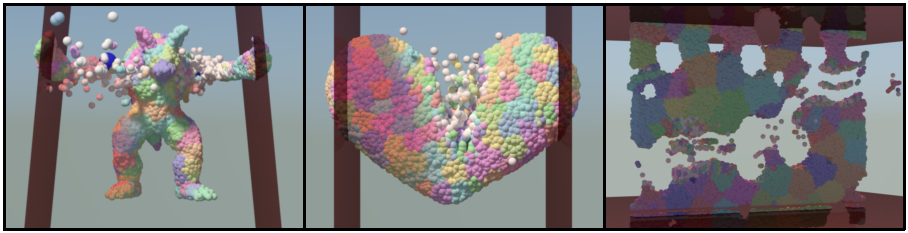
\includegraphics[width=\linewidth]{Figures/teaser}
%   \caption{Left: An armadillo is tortured by being torn apart by the arms while being fired upon by spherical projectiles.  Center: A heartbreaking example.  Right: Tearing a slice of swiss cheese.}
%   \label{fig:teaser}
% }

\maketitle

\begin{abstract}
In this paper, we address clustering and collision detection in the clustered shape matching simulation framework
for deformable bodies.  Our clustering algorithm resembles fuzzy c-means and gives particles weighted membership in clusters.
We then use the weights to divide the particles mass among the clusters, resulting in very even distribution of mass over an 
object.  By design our clustering algorithm also forms spherical clusters yielding exceptionally convenient collision geometry.  We further 
enhance this simple collision proxy with halfspaces to allow for fracture or other simple geometric operations.
The resulting approach is fast, versatile, and simple to implement.
\end{abstract}

\begin{CRcatlist}
  \CRcat{I.3.7}{Computer Graphics}{Three-Dimensional Graphics and Realism}{Animation};
  \CRcat{I.6.8}{Simulation and Modeling}{Types of Simulation}{Animation}.
\end{CRcatlist}

\keywordlist

%% Required for all content. 

\copyrightspace

\section{Introduction}\label{sec:Introduction}
{\em Shape matching} is a geometrically motivated technique for animating deformable bodies introduced
a decade ago by \Mueller and colleagues~\shortcite{Mueller:2005:MDB}.
\fref{fig:shapematching} summarizes the approach.


\begin{figure*}
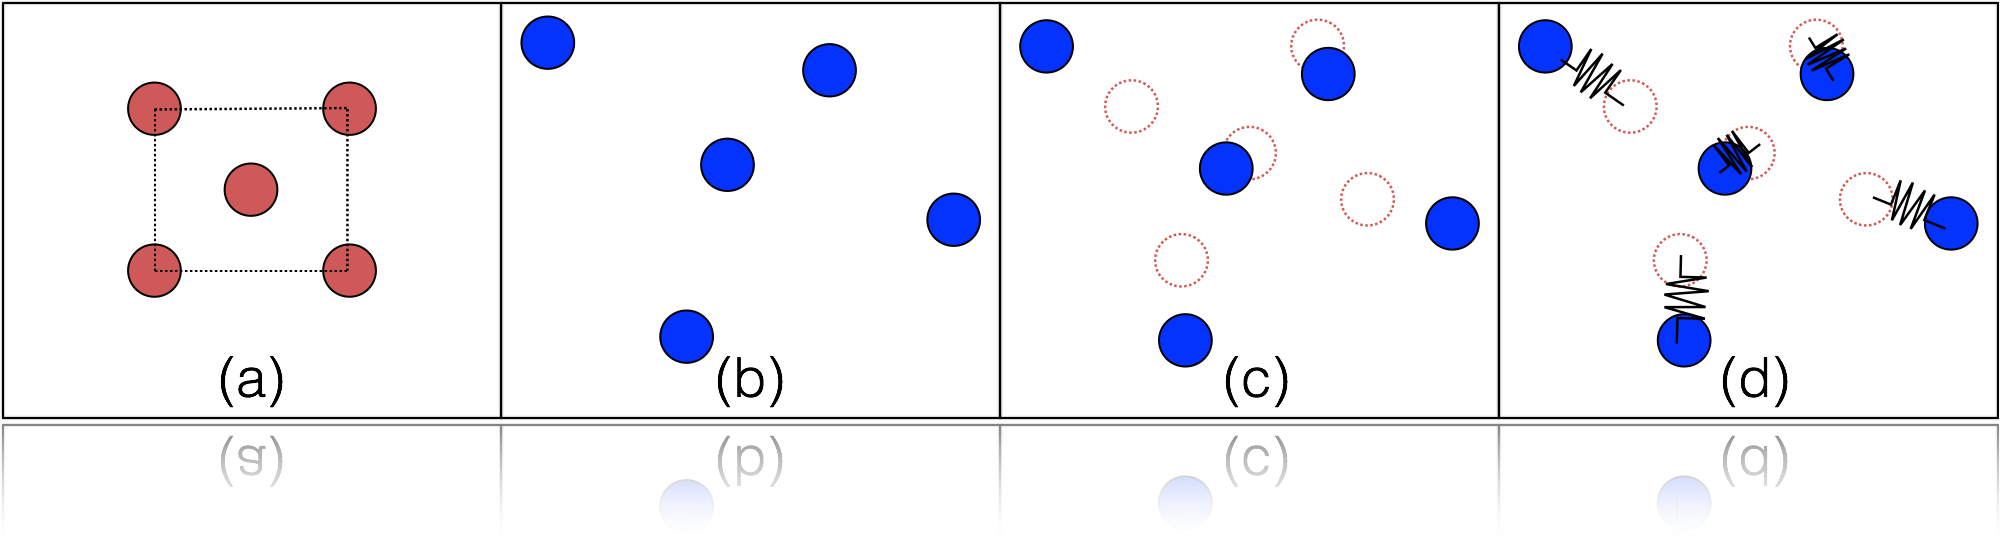
\includegraphics[width=\linewidth]{Figures/shapematching.png}
\caption{Shape Matching Overview: (a) An object (here, a square) is sampled with particles, $p_i$, to get rest positions, $\B{r}_i$.  
(b) As particles are subjected to external forces and constraints, their positions, $\B{x}_i$, are updated in world space.  
(c)  The best-fitting rigid transformation of the particles' rest positions, $\B{r}_i$, 
to their world positions, $\B{x}_i$ is computed.  The dotted red circles are the {\em goal} positions, $\B{g}_i$.  
(d) Hookean springs pull the world positions toward the goal positions.}
\label{fig:shapematching}
\end{figure*}

\section{Related Work}
The geometrically motivated shape matching approach was introduced by \Mueller and 
colleagues~\shortcite{Mueller:2005:MDB}, who demonstrated impressive results and 
described the key advantages of the approach: efficiency, stability, and controllability.
Given these advantages, shape matching is especially appealing in interactive animation contexts such as
video games.  The authors also introduced several extensions including linear and quadratic deformations 
(in addition to rigid deformations), cluster-based deformation, and plasticity.  

Two years later, Rivers and James~\shortcite{Rivers:2007:FFL} introduced lattice-based shape matching,
which used a set of hierarchical lattices to define the shape matching clusters.  They took advantage
of the regular structure of the lattices to achieve extremely high performance.  

Despite impressive results and substantial promise,
the shape matching framework has been largely disregarded by the research community in favor of position-based
dynamics~\cite{Mueller:2007:PBD,Bender:2013:PBM,Bender:2014:ASO,Macklin:2014:UPP}.  One notable exception is
the work of Bargteil and Jones~\shortcite{Bargteil:2014:SLF}, which incorporated strain-limiting into clustered shape matching
and pointed out several advantages of shape matching over position-based dynamics.  Most sifnificantly, shape matching respects Newton's 
laws of motion.

Clustering is well-studied in the machine learning literature and many techniques, such as $\mathrm{k-means}$ , have become standard tools in computer graphics.  
A complete survey of this literature is beyond the scope of this short paper, but for the sort of ``fuzzy'' clustering we propose in this paper,
we recommend the survey by Nock and Nielsen~\shortcite{Nock:2006:OWC}.  Similarly, collision detection is well-studied in the 
computer graphics and robotics literature.  For a survey of real-time techniques we recommend the text by Ericson~\shortcite{Ericson:2004:RCD}.

\section{Methods}
For completeness and readability, we first briefly review the shape matching approach of \Mueller and colleagues~\shortcite{Mueller:2005:MDB}.
\subsection{Shape Matching}
\label{sec:ShapeMatching}
In the shape matching framework
objects are discretized into a set of particles, $p_i\in\mathcal{P}$, with masses, $m_i$, and rest positions, $\B{r}_i$, 
that follow a path, $\B{x}_i(t)$, in world-space through time.  
Shape matching takes its name from the fact that, each frame, we match the rest shape to 
the deformed shape by finding
the least-squares best-fit rigid transformation from the rest pose
to the current deformed pose by
solving for the rotation matrix, $\B{R}$, and translation
vector, $\B{x}_{cm}-\B{r}_{cm}$, that minimizes
\begin{equation}
\label{eq:sm}
\sum_i m_i \| \B{R}\left(\B{r}_i - \B{r}_{cm}\right)-\left(\B{x}_i-\B{x}_{cm}\right)\|^2.
\end{equation}
The best translation is given by the center-of-mass in the rest and world space.  
Computing the rotation, $\B{R}$, is more involved.  
We first compute the least-squares best-fit linear deformation gradient, $\B{F}$.
Specifically, we seek the $\B{F}$ that minimizes
\begin{equation}
\sum_i m_i \| \B{F}\left(\B{r}_i - \B{r}_{cm}\right)-\left(\B{x}_i-\B{x}_{cm}\right)\|^2.
\end{equation}
Setting the derivative with respect to $\B{F}$ to $0$ and re-arranging terms we arrive at
\begin{equation}
\label{eq:defgrad}
\B{F} = \left(\sum_i m_i \B{O}(\B{x}_i,\B{r}_i)\right)\left(\sum_im_i\B{O}(\B{r}_i,\B{r}_i)\right)^{-1} = \B{A}_{xr}\B{A}_{rr}^{-1},
\end{equation}
where $\B{O}(\cdot,\cdot)$ is the outer product matrix
\begin{equation}
\B{O}(\B{a}_i,\B{b}_i) = \left(\B{a}_i-\B{a}_{cm}\right)\left(\B{b}_{i}-\B{b}_{cm}\right)^T,
\end{equation}
and $\B{A}_{**}$ is a convenient shorthand.
%\begin{align}
%\B{F} = &\left(\sum_i m_i\left(\B{x}_{i}-\B{x}_{cm}\right)\left(\B{r}_{i}-\B{r}_{cm}\right)^T\right)\notag\\
%&\left(\sum_i m_i\left(\B{r}_{i}-\B{r}_{cm}\right)\left(\B{r}_{i}-\B{r}_{cm}\right)^T\right)^{-1},
%\end{align}
%and $m_i$ is the mass of $p_i$. 
We then compute $\B{R}$ using the polar decomposition,
\begin{equation}
\label{eq:decomp}
\B{F} = \B{R}\B{S} = \left(\B{UV}^T\right)\left(\B{V\Sigma V}^T\right)
\end{equation}
where $\B{S}=\B{V\Sigma V}^T$ is a symmetric matrix and $\B{U\Sigma V}^T$ is the singular value decomposition (SVD) of $\B{F}$.
While several researchers (e.g.~\cite{Rivers:2007:FFL}) have pointed out that polar decompositions can be computed faster than the SVD,
especially when warm started, the SVD requires a negligible portion of our computation time and, in our experiments, 
the optimized SVD in the Eigen library was faster than our implementations of polar decompositions.  Furthermore, the SVD is more robust in
the presence of degeneracies or inversions.
We also note that we compute the polar decomposition of $\B{F}$, not
the left matrix ($\B{A}_{xr}$)
%($\sum_im_i\B{O}(\B{x}_i,\B{r}_i)$) 
as done by \Mueller and colleagues~\shortcite{Mueller:2005:MDB}.  This modification
is particularly important if the distribution of mass in the cluster is non-uniform and $\B{F}$ is not a pure rotation.

Given $\B{R}$ and $\B{x}_{cm}-\B{r}_{cm}$, we define goal positions, $\B{g}_i$, as
\begin{equation}
\B{g}_i = \B{R}\left(\B{r}_i-\B{r}_{cm}\right)+\B{x}_{cm}.
\end{equation}
Hookean springs are then used to define forces that move the particles toward the goal positions.

\subsection{Clustered Shape Matching}
Handling multiple clusters is straightforward.  When computing a particle's contribution to 
cluster quantities, we must divide the particle's mass among its clusters.  To do 
so we introduce a weight $w_{i,c}$ for particle $p_i$ in cluster $c$ that describes how much of
$p_i$'s mass is contributed to cluster $c$.  These weights enter into equations \eqref{eq:sm}-\eqref{eq:defgrad} by multiplying
the particle's mass.  As an example, the center-of-mass of cluster $c$, $\B{x}_{cm,c} = \B{x}_{c}$ (dropping the $_{cm}$ for clarity), is
\begin{equation}
\label{eq:com}
\B{x}_{c} = \frac{\sum_{p_i\in\mathcal{P}_c}(m_iw_{i,c})~\B{x_i}}{\sum_{p_i\in\mathcal{P}_c}(m_iw_{i,c})}% = \frac{\sum_{p_i\in\mathcal{P}_c}(m_i/n_i) \B{x_i}}{\sum_{p_i\in\mathcal{P}_c}(m_i/n_i)},
\end{equation}
where $\mathcal{P}_c$ is the set of particles in cluster $c$.
We experimented with five weighting schemes in our implementation.  The first, and simplest, weighting
scheme divides the particles mass evenly among the $n_i$ clusters it belongs to, $w_{i,c} = 1/n_i$.
%divide the particle's mass by the number of clusters it belongs to,
%essentially replacing $m_i$ with $m_i/n_i$ in equations \eqref{eq:sm}-\eqref{eq:defgrad} 
%and when computing cluster mass and center-of-mass.
This scheme correspnds to the ``box'' kernel, or constant weights,
\begin{equation}
\label{eq:box}
\mathrm{box}(\B{x}_i, \B{x}_{c}, h) = 1.
\end{equation}
Second is the well-known $\mathrm{poly6}(\cdot)$ kernel~\cite{Mueller:2003:PFS},
\begin{equation}
\label{eq:poly6}
\mathrm{poly6}(\B{x}_i, \B{x}_{c}, h) = \frac{315}{64\pi h^9}\left(h^2-\|\B{x}_i-\B{x}_{c}\|^2\right)^3,
\end{equation}
where $h$ is the kernel width.
Third is a blend of the $\mathrm{box}$ and $\mathrm{poly6}$ kernels
\begin{equation}
\label{blend}
\mathrm{blend}(\B{x}_i, \B{x}_{c}, h) = \beta + \mathrm{poly6}(\B{x}_i, \B{x}_{c}, h),
\end{equation}
where $\beta$ is a blend parameter.
Fourth is a simple inverse distance squared kernel,
\begin{equation}
\label{eq:invdistancesquared}
\mathrm{invsq}(\B{x}_i, \B{x}_{c}, h) = \frac{1}{\|\B{x}_i-\B{x}_{c}\|+\epsilon},
\end{equation}
where $\epsilon$ prevents dividing by zero (we use $\epsilon = 0.0001$).
Fifth is the fuzzy c-means weighting function~\cite{Dunn:1973:AFR,Bezdek:1981:PRF},
\begin{equation}
\label{eq:fuzzycmeans}
\displaystyle \mathrm{fcm}(\B{x}_i, \B{x}_{c}, h) = \dfrac{1}{\displaystyle \sum_{d\in\mathcal{C}}\left(\dfrac{\|x_i - x_{c}\|}{\|x_i-x_{d}\|}\right)^{\tfrac{2}{m-1}}},
\end{equation}
where $m$ is a user-specified parameter greater than one.
Note that $\mathrm{fcm}$ is the only weighting function where the weight in one cluster depends on the positions of other cluster centers,
which significantly complicates computation.

To ensure that the total mass of the clusters equals the total mass of the particles, for all kernels we normalize our weights to a partition of unity,
\begin{equation}
\label{eq:weights}
w_{i,c} = \frac{\mathrm{kernel}(\B{x}_i, \B{x}_{c}, h)}{\sum_{d\in\mathcal{C}}\mathrm{kernel}(\B{x}_i, \B{x}_{d}, h)}
\end{equation}
As discussed in~\sref{sec:results} the choice of kernel can have significant impact on the results; while we selected
$\mathrm{invsq}$ as our default, our implementation makes it easy to switch between kernels to satisfy artistic goals.

%We also essentially replace $m_i$ with $w_{i,c}m_i$ in equations \eqref{eq:sm}-\eqref{eq:defgrad} 
As noted above, these weights show up in many of our calculations.  As another example,
when computing the goal position, $\B{g}_i$, for a particle we perform a weighted
average of the goal positions given by each cluster it is a part of.  That is,
\begin{equation}
\B{g}_i = \sum_c w_{i,c}~\B{g}_{i,c},
\end{equation}
where $\B{g}_{i,c}$ is the goal position for particle $p_i$ in cluster $c$.

\paragraph{Strain Limiting}
To maintain stability we adopt the strain limiting approach advocated by Bargteil and Jones~\shortcite{Bargteil:2014:SLF}.

\subsection{Clustering}
In our context, there are several desirable properities for a clustering algorithm.  Of utmost importance is that the clusters overlap, 
otherwise the simulated object will fall apart.  The clusters must also include all the particles, preferably with a modest number of clusters.  
Finally, if the clusters are well-approximated by spheres, collision handling becomes far simpler.  While clustering is
very well-studied in machine learning, these properties are unique to our problem and we are not aware of any algorithm tailored to these
constraints.  

In our implementation we experimented with three clustering algorithms.  The first algorithm, $\mathrm{random}$,
borrowed from Bargteil and Jones~\shortcite{Bargteil:2014:SLF}, is a simple randomized scheme that iteratively
chooses a random particle that is not a member of any cluster,
uses its location as the center of a new cluster, and adds all particles within a user-specified distance to the cluster.  
The algorithm terminates when all particles are a member of at least on cluster.  Weights, cluster center-of-mass, etc are
determined after the algorithm terminates.  The user can specify the radius of a cluster's neighborhood, but not the number of clusters.

The second algorithm uses $\mathrm{k-means}$ to determine cluster centers; given random seed locations for clusters, this two-step algorithm iteratively
\begin{enumerate}
\item updates cluster membership for each particle by choosing the nearest cluster center;
\item updates cluster centers to be the center of mass of the particles in the cluster.
\end{enumerate}
Convergence is achieved when cluster membership is no longer changing.  
After the $\mathrm{k-means}$ algorithm terminates overlapping clusters are computed by including
all particles within a user-specified distance of the computed cluster centers.  Finally, membership weights, cluster center-of-mass, etc are computed.

Our final approach more closely resembles {\em fuzzy c-means}~\cite{Dunn:1973:AFR,Bezdek:1981:PRF}, 
but explicitly seeks greater sparsity in the membership weights by forcing
weights for particles far from a cluster center to zero.
%Consequently, we developed our own approach, which is quite similar to fuzzy c-means, k-means, expecationa maximization (EM), 
%and Lloyd's algorithm.  Like all these algorithms, 
Again, we iteratively perform two-steps:
\begin{enumerate}
\item update cluster membership {\em and weights};
\item update cluster centers to be the center of mass of the particles in the cluster.
\end{enumerate}
Instead of computing the nearest cluster center for each particle as in $\mathrm{k-means}$, our algorithm includes all particles within a given distance
using a standard spherical range query, which is accelareted with a grid data structure.  Computing the weights 
(\eref{eq:weights}) requires evaluating the above 
kernels for each particle in each cluster and keeping a running sum of the weights for each particle.  Updating the cluster centers simply requires 
computing~\eref{eq:com} for each cluster using the weights computed in the previous step.  To faciliate satisfying the first requirement that 
all particles belong to at least one particle, we add any particles that are not within $h$ of any cluster center to the nearest cluster 
(in a similar manner to the $\mathrm{k-means}$ algorithm).  Any such particles immediately signal that the algorithm has not converged.  Otherwise,
we declare convergence if cluster membership remains the same for two iterations and the cluster centers have not moved more than $0.1\%$ of the neighborhood radius.   
If the algorithm
does not converge within a limited number of iterations we increase the number of clusters and/or $h$ until convergence is achieved.

Compared to $\mathrm{k-means}$ our algorithm has the advantage of including the fact that clusters should overlap in the optimization itself, which leads to slower convergence, but
also to a clustering that is better suited to our needs.

\subsection{Collision Detection}



\section{Results and Discussion}
\label{sec:results}
\begin{table*}
\begin{center}
\caption{Timing results in ms per frame taken on a Macbook Pro with a 2.4Ghz Intel i5 processor.}
\label{table:timing}
\begin{tabular}{|l|l|l|l|l|l|}
\hline
example & \# particles & dynamics & plasticity & fracture & total\\
\hline
armadillo & 20115 & 16  & $<$ 1 & $<$ 1 & 24\\
twisted bar & 5317 & 7 & $<$ 1  & 0 & 7\\
twisted bar with fracture & 5317 & 7  & $<$ 1 & $<$ 1 & 9 \\
projectile & 5325 & 20 & $<$ 1 & $<$ 1 & 29\\
broken heart & 20132 & 22 & $<$ 1 & $<$1 & 31\\
swiss cheese & 25032 & 27 & $<$ 1 & $<$1 & 39 \\
\hline
\end{tabular}
\end{center}
\end{table*}

\paragraph{Limitations and Future Work}

Our blue-noise sampling and $\mathrm{k-means}$ clustering improve upon the regular grids and
randomized clusters of Bargteil and Jones~\shortcite{Bargteil:2014:SLF} and are effective for our purposes,
but better approaches certainly exist.  In particular, it would be interesting to explore adaptive sampling
so that computational resources can be focused on interesting areas of the object.  
Changing the sampling over time as done by Pauly and colleagues~\shortcite{Pauly:2005:MAO}
is also a promising avenue for future work, which may help address the geometric limitations discussed above.
It would also be interesting
to consider adaptive and hierarchical clustering techniques; the hierarchical lattices of Rivers and James~\cite{Rivers:2007:FFL}
clearly improved performance and artistic directability.  

The biggest limitation of our approach is a lack of theoretical underpinnings for the clustered shape matching
framework; we do not yet have any mathematical tools to analyze the approach.  We do not really understand
how the method behaves as particle counts or timesteps decrease or as the cluster size or number of clusters change.
This limitation does not mean the approach is not useful.  After all, the finite element method was in use
for decades before a mathematical framework was developed to analyze its properties.  In a similar way,
we believe the clustered shape-matching framework will prove extremely useful in practice while
researchers develop mathematical tools for analysis. 

\paragraph{Conclusion} 
One of the primary advantages of the clustered shape matching approach is that the number of degrees of freedom
is much larger then the number of ``integration units''---clusters in this case.  The opposite is true of finite element
methods with unstructured meshes where the number of tetrahedra is often considerably larger than the number of vertices.  
For graphical applications visual detail, which correlates with the number of degrees of freedom, is of paramount importance
and computation, which correlates with ``integration units,'' is often limited.  
For these reasons, the clustered shape matching framework is extremely appealing for computer animation, 
especially interactive animation.  The utility and versatility of this framework is greatly improved by our extensions 
to clustering and collision handling.




\section*{Acknowledgements}
Removed for anonymous review.

\bibliographystyle{acmsiggraph}
\bibliography{csm}
\end{document}
